\chapter{Introduction}

\section{Project objectives and overview}
The aim of this Thesis, partially funded by the Allianz Insurance Company, is to produce riverine flood risk maps over the complete Italian domain for both the present day climate and for future projections. Due to the requirements of a strictly physically-based reproducible scientific approach, a framework consisting in a model chain of three tried-and-tested models, spanning climate, hydrology, and hydraulics, was developed. This Thesis thus describes a truly inter-disciplinary approach to flood risk modelling.

In order to obtain a reliable representation of flood risk, model calibration and evaluation was performed using several observational datasets of precipitation, discharge and flood extent. In particular, a new gridded hourly precipitation dataset for the complete Italian territory was developed in conjunction with the University of L'Aquila. The development of such dataset represents a necessary step in the scientific process described in this Thesis since, to our knowledge, no database suitable for driving a high-resolution hourly hydrological model is currently available over Italy.\\

\subsection{The structure of this Thesis}
DESCRIBE HOW IS THIS THESIS ORGANISED

\section{Flood hazard estimation: an overview} \label{sec:flood_overview}
Floods are some of the most devastating natural disasters, with strong impacts on both the societal and economic scale. According to the Centre for Research on the Epidemiology of Disasters (\cite{Guha-sapir2011}), several thousand people are killed every year by floods worldwide, with an average of about 5700 deaths in the period 2006--2015 and 82.6 million people affected every year. Flood-related damages, amounting to \SI{34}[\$]{G} yearly, account for one third (\cite{MunichRE}) to one quarter (\cite{Guha-sapir2011}) of the total disaster damage claimed worldwide, with damages amounting to \SI{15.45}[\$]{G} in the USA alone in 2016. For Europe in particular, floods have caused about \SI{100}[\€]{G} in damages in the period 1986--2006 (\cite{Cea2007}).

For these reasons, flood forecasting and risk estimation are an essential tool for protecting the population from flood-related damages both financially, via insurance policies, and physically, via water management and engineering.

\subsection{Different kinds of floods; flood risk and flood hazard, Return Period}
According to the European Union Floods Directive a flood is defined by the \enquote{temporary covering by water of land not normally covered by water} (\cite{EUFD2007}).
Three main types of floods are usually recognised (see \cite{Kron2005}), with each having its own characteristics:
\begin{itemize}
    \item[Storm surge] can occur when low pressure systems, strong winds and/or high tides combine to cause high waters in coastal areas. This type of floods is especially frequent in regions where strong cyclonic development can easily take place.
    \item[Flash floods] are extremely fast floods that are characterised by a short timescale, usually below 6 hours. They can be caused by very strong, sudden precipitation, especially in urban areas, or by artificial events, such as dam failure.
    \item[River floods] associated with unusually strong and persistent precipitation and snow melt, are instead characterised by a longer life cycle, up to several days. They are usually caused by the gradual increase in river discharge, up to the point where water level overtops levees or overflows river banks. The time scale of riverine floods is usually dependant on the size of the catchment This is the type of floods which will be considered by this work.
\end{itemize}

One important distinction to make is the one between flood risk and flood probability (or hazard).\\
Risk is usually defined (see e.g. , \cite{Kron2002, DeMoel2009}, \cite{Merz2007}) as the product of the probability of an event happening and its possible consequences. The latter factor can be further split into two different aspects: exposure and coping factor, so that:
$$\text{RISK} = \underbrace{\text{HOW OFTEN}}_\text{RETURN PERIOD} \times \underbrace{\text{WHAT} \times \text{HOW}}_\text{CONSEQUENCES}$$
Exposure (the "WHAT") relates to the physical and societal goods at risk; the coping factor (the "HOW") instead relates to which extent a given area is capable of dealing with the effects of a flood.\\
While policymakers tend to focus the efforts of risk mitigation primarily towards the reduction of the latter terms, in this Thesis we are primarily concerned with flood probability (the "HOW OFTEN"), usually measured by its Return Period (or Recurrence Interval):
$$\frac{\text{period length} + 1}{\text{number of events}}$$
Statistically, the Return Period (RP) can be considered as the inverse of the probability that the event will occur in any year. As an example, a 100--year flood is a flood that has a probability of occurring of $1\%$ in any given year.

\subsection{Methods of flood hazard estimation}\label{subs:flood_hazard_methods}
Different kinds of flood maps are usually produced with different methods by governments, regional agencies, or insurance and re-insurance companies (\cite{DeMoel2009}). The resulting fragmentation often makes it hard to distinguish between solid, scientifically-based approaches and less reliable methods, especially since the level of uncertainty is rarely provided. Especially for private companies, the methods and input data used for obtaining flood maps are often undisclosed, resulting in products that cannot be considered scientifically-based and reproducible.\\

Historically speaking, flood risk was estimated via the analysis of historical discharge and flooding records and by surveying local people; the statistical analysis of these observations can however be misleading, as extreme floods are extremely rare events and long observational periods, in excess of a few tens of years, have little chance of being available. This major limitation can be partially addressed by researching into documentary evidence of past floods (\cite{Kjeldsen2014}, \cite{Reed2002}), but these are often equally hard to come by and can be hard to properly interpret.\\

In the last decades, however, new approaches based on hydrological and hydraulical modelling emerged as viable. In this multimodel approach a hydrological simulation, driven by precipitation data, generates discharge data for a given region or basin for a long period of time; this discharge  is then fed to a second hydrodynamic model which reproduces hypothetical flood extents and, if necessary, other variables such as flood depth or flow speed.\\
Extreme value analysis can also be applied to the discharge output, assuming a given distribution for extreme events. This allows to extend the analysis of shorter observational records to long Return Periods of 100 years or more. This process has the advantage of being very flexible, potentially requiring precipitation data instead of discharge data, which are generally less readily available. Additionally, using precipitation data from large scale datasets, this technique can work on virtually any domain, including ungauged ones, which opens the door for multi-regional and cross-catchement analysis.\\

There are downsides to this approach too: a large amount of observational data, for calibration and evaluation, is still advisable; moreover, having a model working off another model's output, in a chain, can make the estimation of the uncertainty of the final output harder. One more important source of uncertainty is the generally followed assumption that flood defences and river levees and banks will not fail; additionally, for heavily managed rivers, water management can prevent flooding by diverting additional water to reservoirs, other rivers, or agricultural areas, which is usually unaccounted for.

\subsection{Different kinds of flood maps} \label{sec:flood_map_types}
As highlighted in the previous section, the generic term \enquote{flood maps} can refer to several different products, from historical "flooded point" references to economic risk maps. \cite{DeMoel2009} presents a nice overview of 6 different types (Figure \ref{fig:flood_map_types}):

\begin{enumerate}[label=\Alph*] %uses pkg {enumitem}
\item Flooded points in historical records
\item Flooded area probability, each year, for different Return Periods (10, 100 and 500 years)\label{enum:RP_map}
\item Flooded area water depth for a given Return Period
\item Qualitative flood danger, usually calculated as a combination of Return Period, depth, flow speed or other factors
\item Qualitative flood risk, including information on population density and other societal variables
\item Quantitative flood risk, showing information on direct economic damage
\end{enumerate}

In this Thesis work the focus is on producing Return Period and flood depth maps, which are generally considered the most important variables in flood hazard estimation.

\begin{figure}[h]
    \centering
    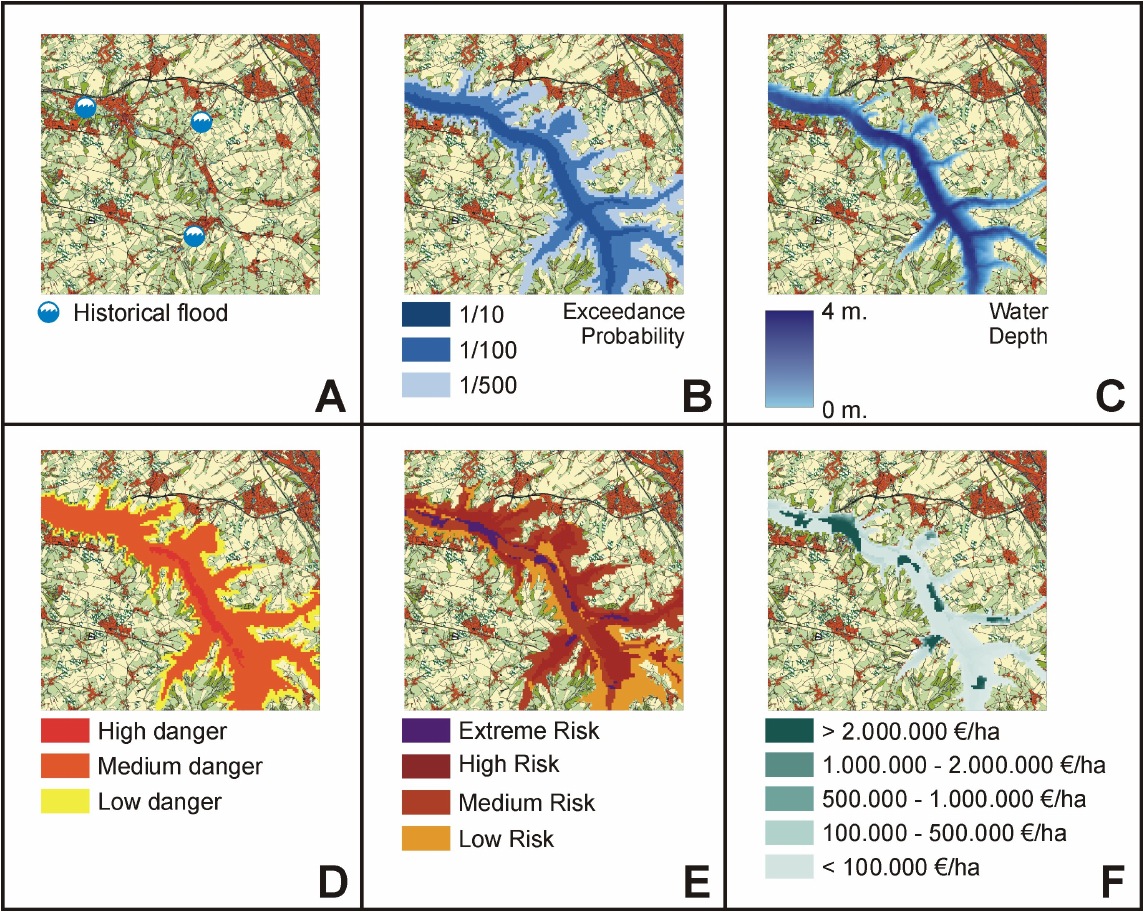
\includegraphics[width=\textwidth]{figures/flood_map_types}
    \decoRule
    \caption[Flood map types]{A depiction of 6 different flood map types, from  \cite{DeMoel2009}, Figure 2. Refer to section \ref{sec:flood_map_types} for description of the panels}
    \label{fig:flood_map_types}
\end{figure}

\section{The climatological-hydrological-hydraulical approach}
The flood hazard estimation method developed in this project follows the footsteps of similar approaches as depicted in section \ref{subs:flood_hazard_methods}: an hydrological model, driven by observations or by a Regional Climate Model, reproduces discharge data over several different Italian domains and for a period of several years; these discharges are then fitted statistically to an extreme value distribution which allows to extends the simulation of extreme events to any Return Period, with decreasing accuracy as the rarity of the event increases. The typical discharge for a selected number of Return Periods for each point is then modelled via an hydraulical model to produce flood extent maps. In our case, the procedure is based on the work of \cite{PAPER_MAIONE?}, who performed a similar analysis, starting strictly from observational data, for the Po river basin ***CHECK THIS, REREAD PAPER***.

This procedure, as shown in the following chapters, was applied both with observational data and with data coming from a Regional Climate Model, in an off--line nesting setup. For the time being only domains covering the complete Italian territory were simulated, but no limitation is in place that would prevent this technique to be applied to any domain worldwide.


\section{The future of extreme climatological and hydrological events}
The Earth is currently undergoing a relatively rapid warming period which is, according to climate scientists, primarily linked to antropogenic activity (\ref{Anderegg2010, IPCC2013}). Climate change affects all aspects of the atmospheric system, including the events which are usually associated with floods, such as extremely strong or prolonged periods of rain. Physical constraints suggest that increasing heavy precipitations are more correlated with the total amount of moisture in the air (growing by approximately 7\% per \SI{}{\celsius} according to the Clausius-Clapeyron equation) than with changing in mean precipitation (\cite{Allen2002}), leading to the observation that increases in extreme rainfall might happen even in regions with decreasing total precipitation. In fact, numerous studies (e.g. \cite{Frei2006a, Christensen2004, Rajczak2013a, Pal2004, Durman2001, KleinTank2003, Fowler2003}) have shown high likelihood of increasing frequency and/or intensity of such events before the end of the century, even in regions where the total precipitation is supposed to decrease.\\
The evidence over Europe is particularly overwhelming, which suggests that Europe is one of the regions which is more exposed to climate change (\ref{giorgi2006Clichahot}).

As for flooding, flood risk is expected to strongly increase worldwide, continuing a trend that has already been detected in recent decades. The exposure and damage numbers given at the beginning of Section \ref{sec:flood_overview} are destined to increase, despite improving flood protection infrastructures, primarily due to higher exposure (\cite{MunichRE2015, Kron2005, Hirabayashi2009, Mitchell2003}) in flood-prone areas, which are on average very attractive for socio--economic activities.\\
\cite{Jongman2012} calculated that the total exposure to flood disasters, which is reported at \$\SIrange{27}{46}{T} globally in 2010, is going to more than triple (to \$\SIrange{80}{158}{T}) in 2050. In Europe, according to some studies (\cite{Rojas2013, Alfieri2015}), the current annual population affected is expected to significantly by the 2080s, with annual damages growing up to 20--fold, if no change occurs in the current climate mitigation politics.

The strongest driver for increasing flood risk is, however, high exposure due to, primarily, growing population density. The other main factor, flood hazard, is also generally projected to increase according to the majority of studies. The outcome is however very dependant on the region or even basin of interest, as local flood-related climatic characteristic can differ greatly from one region to another. Global studies (\cite{Hirabayashi2013, Arnell2016, Dankers2014, Hirabayashi2008, Alfieri2017, Milly2002}), for example, generally find definite increasing likelihood of flood events in the future for Southern Asia, Western Russia, Canada and the Northern Andes, but decreasing likelihood for Western Europe and the Amazon Basin. The resolution of such large scale studies, however, is usually not fine enough to resolve the details of most river catchments (\cite{Whitfield2012, Gosling2011}), especially for European basins, which are typically small in size.\\
Smaller scale studies (e.g. \cite{Dankers2009, Alfieri2015a, Prudhomme2003}) over the European continent (or single European countries) generally find increasing flood hazard in most basins, especially in terms of higher frequency more than of higher magnitude (\cite{Alfieri2015a, Lehner2006}), but large regional variations can be found (\cite{Rojas2012}) due to the very different climatic characteristics of the region. As can be expected, the changes generally show strong seasonality, with increased discharges and frequency of flood events mostly concentrating in autumn and winter (e.g. \cite{Middelkoop2001}).

\subsubsection{*** some papers to be integrated above follow ***}
\begin{itemize}
    \item  On a smaller, catchment scale, \cite{Cloke2013} find increased flood hazard for the Upper Severn basin, but highlight potential differences when using different methodologies and models, arguing an ensemble approach would be more reliable, given the large uncertainties inherent to reproducing extreme events in a model chain.
    \item A lot of studies (e.g. Dankers2009, Alfieri2017, Kay2009, Gosling2011, Bell2007, Prudhomme2003) highlight that a multimodel ensemble is way better... I should explain why this was unattainable in our case
    \item Gosling2011 looks at the difference between catchement scale hydrological models and global hydro models
    \item
\end{itemize}








\section{Additional sources to integrate in this chapter}
\begin{enumerate}
    \item \cite{DeMoel2009} gives a nice overview of several methods, and a nice introduction on the current (well, 9 years ago) EU legislation. Also, a good source for the definition of "risk". <- read this again
    \item might want to add figure 1 from DeMoel2009
    \item Plate2002 is an excellent overview on how to handle risk managment, which is not extremely interesting for us
    \item \cite{Arnell2016} gives a very good overview of projected flood risk in climate change, also includes a LONG list of papeers which might be interesing
    \item AR5 WG1 (\cite{IPCC2013}), p134, figure 1.8 -> very nice ; see also 2.6.2, specifically 2.6.2.2
    \item See also 23.3.1.2. River and Pluvial Flooding and from \cite{Aalst2014}
\end{enumerate}